% !TEX root = ../Ausarbeitung.tex
\section{Containertechnologien} 
\label{sec:Containertechnologien}

In der Geschichte der Containertechnologie traten verschiedene Implementierungsformen auf.
Hierbei waren die ersten Umsetzungen noch sehr einfach aufgebaut und wurden mit den Anforderungen an die Containerdienste immer komplexer.
Im Folgenden findet sich eine Übersicht über die wichtigsten Technologien der Containerisierung.

\begin{figure}[H]
	\begin{center}
		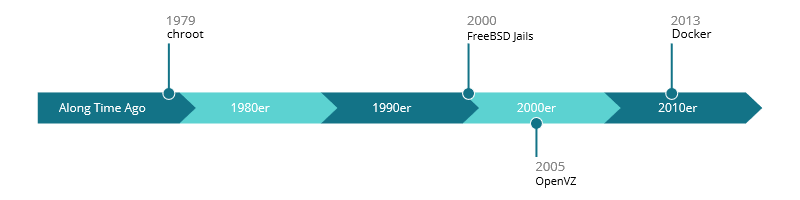
\includegraphics[width=0.8\textwidth]{ZeitContainer.png}
	\end{center}
	\caption[Containertechnologie im Laufe der Zeit]{Containertechnologie im Laufe der Zeit}
	\label{fig:CTZeit}
\end{figure}


\subsection{chroot}
\label{sec:chroot}

Chroot ist ein Befehl, der schon früh in Unix-Systemen eingebaut wurde.
Er ermöglicht es einem Prozess, ein anderes Rootverzeichnis zu geben.
Wird in einem Programm \code{chroot()} aufgerufen, wechselt es das Verzeichnis und kann nicht auf Dateien außerhalb der zugewiesenen Struktur zugreifen.
Diese Abschottung eines Prozess war nie als Sicherheitsfeature vorgesehen und wird hauptsächlich zur Virtualisierung eingesetzt.
Mit dem Befehl können einzelne Prozesse auf Dateiebene von anderen Anwendungen getrennt werden, weitere Sicherheitsmechanismen oder Isolierungen gibt es nicht.\cite{IEEE7830207,569694, MANPAGE01}

\subsection{OpenVZ}
\label{sec:OpenVZ}

Im Jahr 2005 veröffentlichte die Firma SWsoft (später umbenannt zu Parallels) ihr Projekt OpenVZ unter der GNU GPL Lizenz. OpenVZ basierte auf der Idee der Container, ermöglicht es jedoch in jedem Container eine eigene Linux-Distribution auszuführen.
Die durch die Containerumgebung abgegrenzten Betriebssysteme, teilen sich dabei einen Kernel. Dadurch ist der Overhead von OpenVZ deutlich geringer als bei der klassischen Vollvirtualisierung eines Betriebssystems.
In den einzelnen Containern gibt es jeweils einen eigenen root-User und eine eigene Dateistruktur.
Sie können unabhängig voneinander gestarten und gestoppt werden.
Da sich die Betriebssysteme einen Kernel teilen, können auch die Gastsysteme nur Linux-Systeme sein.
Da viele der Änderungen von OpenVZ den Kernel von Linux betreffen, werden regelmäßig Änderungen von OpenVZ-Patches in den Kernel von Linux übernommen.\cite{OpenVzNews, IEEE4803091,OpenVzHist}


\subsection{FreeBSD jails}
\label{sec:jails}



\subsection{LXC}
\label{sec:lxc}

LXC ist seit der erstmaligen Veröffentlichung 2008 ein offizielles Kernelfeature und in den meisten Distributionen von Linux enthalten. Die Abkürzunhg LXC ist eine User Space-Schnittstelle für die erstellung von isolierten Umgebungen innerhalb eines Systems. Dies geschieht durch die Nutzung von Kernel namespace, Apparmor und SELinux-Profilen sowie chroots und cgroups. Diese Features standen schon vor LXC zur Verfügung, jedoch vereinigte sie LXC zu einer Schnittstelle für die Erzeugung von Containern. Zu Beginn der Entwicklung von LXC war die Isolation der Container nicht so gut, sondern glich eher einer Abwandlung der chroot-Funktion. Mit der Zeit wurde die Abschottung jedoch immer besser und die LXC-Container wurden zu richtigen virtualisierten Umgebungen. Dies geschah unter anderem dadurch, dass ab Version 1.0 die einzelnen Container als unpriviliegierte Benutzter ausgeführt werden können. Zuvor war dies nicht möglich und eine Abgrenzung der Container nur bedingt gegeben. LXC ist eine Technologie, die von vielen weiteren Projekten eingesetzt wird, unter anderen auch Proxmox oder Docker (bis Version 1.1)\cite{LXCHomepage,IEEE7036275, IEEE7185212, IEEE7571957,IEEE7929714}


\subsection{LXD}
\label{sec:lxd}

Um die Verwendung von LXC zu vereinfachen wurde das Tool LXD entwickelt. Es besteht aus drei Elementen: Einem Deamon, der eine REST-API zur Verfügung stellt, einem Befehlszeilenclient sowie einem Open-Stack Nova Plugin. Die vom Deamon bereit gestellte Schnittstelle ermöglicht es, über das Netzwerk auf das Management der Container zuzugreifen. LXD ist somit eine Erweiterung, die eine Schnittstelle zu LXC-Containern schafft. Über das Nova Plugin können die einzelnen LXD-Maschinen als Rechenknoten verwendet werden. \cite{LXDHomepage}

\subsection{Solaris Container}
\label{sec:solariscontainer}




\subsection{Windows Containers}
\label{sec:WindowsContainers}



\subsection{Docker}
\label{sec:Docker}



\subsection{Mesos}
\label{sec:Mesos}



\subsection{rkt}
\label{sec:rkt}
